% {{{
\documentclass[12pt]{article}
\usepackage[tmargin=0.75in,bmargin=0.75in,lmargin=0.9in,rmargin=0.9in]{geometry}

\usepackage{amsmath}
\include{latexsym}
\include{amssymb}
\usepackage{enumitem}
\usepackage[symbol, hang]{footmisc}
\usepackage{indentfirst}
\usepackage{amssymb}
\usepackage{graphicx,psfrag}

\def\F{\mathcal{F}}
\def\M{\mathcal{M}}
\def\dimspec{\mathfrak{D}}
\def\htop{h_{top}}
\def\trans{\mathcal{T}}
\def\G{\mathcal{G}}
\newcommand{\Z}{\mathbb{Z}}
\pagenumbering{gobble}
\def\O{\mathcal{O}}

\newcommand\NoIndent[1]{%
  \begingroup
  \par
  \parshape0
  #1\par
  \endgroup
}
% }}}

% Title {{{
\begin{document}

\begin{center}
{\large \bf Comp Methods }   \\ \large Pset 5 \\ Ephraim Sutherland
\end{center}
% }}}

\subsection*{Problem 1}

\begin{enumerate}

	\item we construct two valuation functions
		\begin{align*}
			v_g (k) &= \max_{k'} [ u(z_g k^{\alpha} + (1 - \delta) k - k') + \beta ( \pi_{gg} v_g (k') + \pi_{gb} v_b (k')) ]
		\end{align*} 
		and 
		\begin{align*}
			v_b (k) &= \max_{k'} [ u(z_g k^{\alpha} + (1 - \delta) k - k') + \beta ( \pi_{bg} v_g (k') + \pi_{bb} v_b (k')) ]
		\end{align*} 
		To do this, solve
		\begin{align*}
	 &\max_{k'} [ u(z_g k^{\alpha} + (1 - \delta) k - k') + \beta ( \pi_{gg} v_g (k') + \pi_{gb} v_b (k')) ] \\
	 &\max_{k'} [ \log(z_g k^{\alpha} + (1 - \delta) k - k') + \beta ( \pi_{gg} ( \gamma_{0g} + \gamma_1 \log (k')) + \pi_{gb}(\gamma_{0b} + \gamma_1 \log (k'))) ]
		\end{align*} 
		Using our F.O.C, letting $\delta = 1$ and substituting in our probabilities:
		\begin{align*}
			\frac{-1}{z_g k^{\alpha}   - k'} + \frac{\beta \gamma_1 \pi}{k'} + \frac{\beta ( 1- \pi) \gamma_1}{k'} =0 \\
			\iff \frac{\beta \gamma_1}{k'} = \frac{1}{z_g k^{\alpha}  - k'} \\
				\iff k' = \frac{\beta \gamma_1z_g k^{\alpha}  }{(1 + \beta \gamma_1 )}
				\end{align*} 
				Plugging back into our felicity function.
				% {{{
				\begin{align*}
					v(a) &= \log(z_g k^{\alpha}   - k') + \beta ( \pi_{gg} ( \gamma_{0g} + \gamma_1 \log (k')) + \pi_{gb}(\gamma_{0b} + \gamma_1 \log (k'))) \\
					     &=\log(z_g k^{\alpha}   - \frac{\beta \gamma_1z_g k^{\alpha}  }{(1 + \beta \gamma_1 )}) + \beta ( \pi_{gg} ( \gamma_{0g} + \gamma_1 \log (\frac{\beta \gamma_1z_g k^{\alpha}  }{(1 + \beta \gamma_1 )})) + \pi_{gb}(\gamma_{0b} + \gamma_1 \log (\frac{\beta \gamma_1z_g k^{\alpha}  }{(1 + \beta \gamma_1 )} \\
					     &=\log(\frac{z_g k^{\alpha}  }{(1 + \beta \gamma_1 )}) + \beta ( \pi_{gg} ( \gamma_{0g} + \gamma_1 \log (\frac{\beta \gamma_1z_g k^{\alpha}  }{(1 + \beta \gamma_1 )})) + \pi_{gb}(\gamma_{0b} + \gamma_1 \log (\frac{\beta \gamma_1z_g k^{\alpha}  }{(1 + \beta \gamma_1 )}))) \\
					     &=\log(z_g) + \log( k^{\alpha})  - \log(1 + \beta \gamma_1 ) \\
					     &\quad + \beta \pi_{gg} \gamma_{0g} + \beta \pi_{gg} \gamma_1 \log (\beta \gamma_1z_g) + \gamma_1  \beta \pi_{gg}\log( k^{\alpha}) - \gamma_1 \beta \pi_{gg} \log(1 + \beta \gamma_1 ) \\
					     &\quad + \beta \pi_{gb}\gamma_{0b} + \beta \pi_{gb} \gamma_1 \log (\beta \gamma_1z_g ) + \beta \pi_{gb} \gamma_1 \log(k^{\alpha}) - \beta \pi_{gb} \gamma_1 \log(1 + \beta \gamma_1 ) \\
					     &=\log(z_g)  - \log(1 + \beta \gamma_1 ) \\
					     &\quad + \beta \pi_{gg} \gamma_{0g} + \beta \pi_{gg} \gamma_1 \log (\beta \gamma_1z_g) - \beta \pi_{gg} \gamma_1 \log(1 + \beta \gamma_1 ) \\
					     &\quad + \beta \pi_{gb}\gamma_{0b} + \beta \pi_{gb} \gamma_1 \log (\beta \gamma_1z_g ) - \beta \pi_{gb} \gamma_1 \log(1 + \beta \gamma_1 ) +( \alpha + \gamma_1  \beta \alpha (\pi_{gg}+ \pi_{gb}) \log(k)  \\
					     &=\log(z_g)  - \log(1 + \beta \gamma_1 ) \\
					     &\quad + \beta \pi  \gamma_{0g} + \beta \pi  \gamma_1 \log (\beta \gamma_1z_g) - \beta \pi  \gamma_1 \log(1 + \beta \gamma_1 ) \\
					     &\quad + \beta (1 - \pi) \gamma_{0b} + \beta (1 - \pi)  \gamma_1 \log (\beta \gamma_1z_g ) \\
					     &\quad - \beta (1 - \pi)  \gamma_1 \log(1 + \beta \gamma_1 ) +( \alpha + \gamma_1  \beta \alpha (\pi + (1 - \pi) )) \log(k)  \\
					     &=\log(z_g)  - \log(1 + \beta \gamma_1 ) \\
					     &\quad + \beta \pi  \gamma_{0g} + \beta \pi  \gamma_1 \log (\beta \gamma_1z_g) - \beta \pi  \gamma_1 \log(1 + \beta \gamma_1 ) \\
					     &\quad + \beta (1 - \pi) \gamma_{0b} + \beta (1 - \pi)  \gamma_1 \log (\beta \gamma_1z_g ) \\
					     &\quad - \beta (1 - \pi)  \gamma_1 \log(1 + \beta \gamma_1 ) +( \alpha + \gamma_1  \beta \alpha ) \log(k)  \\
					     &=\log(z_g)  - \log(1 + \beta \gamma_1 ) \\
					     &\quad + \beta \pi  \gamma_{0g} + \beta \gamma_1 \log (\beta \gamma_1z_g) - \beta \gamma_1 \log(1 + \beta \gamma_1 ) \\
					     &\quad + \beta (1 - \pi) \gamma_{0b} + ( \alpha + \gamma_1  \beta \alpha ) \log(k) 
				\end{align*} 
				% }}}
				It's thus clear that 
				$\gamma_1' = ( \alpha + \gamma_1  \beta \alpha ) $
Thus, setting
\begin{align*}
	\gamma_1 = \gamma_1' &= \alpha + \gamma_1  \beta \alpha \\
	\gamma_1' &= \frac{\alpha}{(1 - \alpha \beta )}
\end{align*} Furthermore, 
				\begin{align*}
					\gamma_{0g}' &= \log(z_g)  - \log(1 + \beta \gamma_1 ) + \beta \pi  \gamma_{0g} + \beta \gamma_1 \log (\beta \gamma_1z_g) - \beta \gamma_1 \log(1 + \beta \gamma_1 ) + \beta (1 - \pi) \gamma_{0b} \\
					\intertext{ let $\gamma_{0g}' = \gamma_{0g}$ then we get }
					\gamma_{0g} (1 - \beta \pi ) &= \log(z_g)  + \log(1 - \alpha \beta  ) + \frac{\alpha \beta}{1 - \alpha \beta} \log (\beta z_g \alpha)  + \beta (1 - \pi) \gamma_{0b} \\
				\end{align*}
				by symmetry, (and letting $\gamma_{0b}' = \gamma_{0b}$) we can also see that 
				\begin{align*}
					\gamma_{0b}' &= \log(z_b)  - \log(1 + \beta \gamma_1 ) + \beta \pi  \gamma_{0b} + \beta \gamma_1 \log (\beta \gamma_1z_b) - \beta \gamma_1 \log(1 + \beta \gamma_1 ) + \beta (1 - \pi) \gamma_{0g} \\
					\gamma_{0b} (1 - \beta \pi ) &= \log(z_b)  + \log(1 - \alpha \beta  ) + \frac{\alpha \beta}{1 - \alpha \beta} \log (\beta z_b \alpha)  + \beta (1 - \pi) \gamma_{0g} \\
				\end{align*}
\\
Thus we are left with a system of equations.
Solving $\gamma_{0b}$ and $\gamma_{0g}$ respectively, we get.

\begin{align*}
	\gamma_{0g} (1 - \beta \pi ) &= \log(z_g)  + \log(1 - \alpha \beta  ) + \frac{\alpha \beta}{1 - \alpha \beta} \log (\beta z_g \alpha)  + \beta (1 - \pi) \gamma_{0b} \\
	\gamma_{0b} (1 - \beta \pi ) &= \log(z_b)  + \log(1 - \alpha \beta  ) + \frac{\alpha \beta}{1 - \alpha \beta} \log (\beta z_b \alpha)  + \beta (1 - \pi) \gamma_{0g} 
\end{align*} 
which can be rearranged like
\begin{align}
	0 &= \frac{\log(z_g) }{(1 - \beta \pi )} + \frac{\log(1 - \alpha \beta  )}{(1 - \beta \pi )} + \frac{\alpha \beta}{(1 - \alpha \beta)(1 - \beta \pi )} \log (\beta z_g \alpha)  + \frac{\beta (1 - \pi)}{(1 - \beta \pi )} \gamma_{0b} - \gamma_{0g} \\
	0 &= \frac{\log(z_b) }{(1 - \beta \pi )} + \frac{\log(1 - \alpha \beta  )}{(1 - \beta \pi )} + \frac{\alpha \beta}{(1 - \alpha \beta)(1 - \beta \pi )} \log (\beta z_b \alpha)  + \frac{\beta (1 - \pi)}{(1 - \beta \pi )} \gamma_{0g} - \gamma_{0b} 
\end{align} 
taking  (1) + $\frac{1 - \beta \pi}{\beta - \beta \pi}$ (2)
gives us
\begin{align*}
	0 &= \frac{\log(z_g) }{(1 - \beta \pi )} + \frac{\log(1 - \alpha \beta  )}{(1 - \beta \pi )} + \frac{\alpha \beta}{(1 - \alpha \beta)(1 - \beta \pi )} \log (\beta z_g \alpha)  + \frac{\beta - \beta \pi }{(1 - \beta \pi )} \gamma_{0b} - \gamma_{0g} \\
	  &+ \frac{\log(z_b) }{( \beta - \beta \pi )} + \frac{\log(1 - \alpha \beta  )}{( \beta - \beta \pi )} + \frac{\alpha \beta}{(1 - \alpha \beta)( \beta - \beta \pi )} \log (\beta z_b \alpha)  + \gamma_{0g} - \frac{1 - \beta \pi}{\beta - \beta \pi} \gamma_{0b} \\
	0 &= \underbrace{\frac{\log(z_g) }{(1 - \beta \pi )} + \frac{\log(1 - \alpha \beta  )}{(1 - \beta \pi )} + \frac{\alpha \beta}{(1 - \alpha \beta)(1 - \beta \pi )} \log (\beta z_g \alpha)}_{\tau_1} \\ 
	  &+ \underbrace{\frac{\log(z_b) }{( \beta - \beta \pi )} + \frac{\log(1 - \alpha \beta  )}{( \beta - \beta \pi )} + \frac{\alpha \beta}{(1 - \alpha \beta)( \beta - \beta \pi )} \log (\beta z_b \alpha)}_{\tau_2}  - \frac{1 - \beta \pi}{\beta - \beta \pi} \gamma_{0b} + \frac{\beta - \beta \pi }{(1 - \beta \pi )} \gamma_{0b} \\
\end{align*} 


then we can solve for $\gamma_{0b}$ 
\begin{align*}
	\frac{1 - \beta \pi}{\beta - \beta \pi} \gamma_{0b} - \frac{\beta - \beta \pi }{(1 - \beta \pi )} \gamma_{0b} &= \tau_1 + \tau_2 \\
	\gamma_{0b} \left(\frac{1 - \beta \pi}{\beta - \beta \pi} - \frac{\beta - \beta \pi }{(1 - \beta \pi )} \right) &= \tau_1 + \tau_2 \\
	\gamma_{0b} &= \left(\frac{(\beta - \beta \pi)(1 - \beta \pi)}{(1 - \beta \pi)^2 - (\beta - \beta \pi)^2} \right) (\tau_1 + \tau_2 )\\
\end{align*} 

Finally, we can solve for $\gamma_{0g}$ plugging back into (1)
\begin{align*}
	\gamma_{0g} &= \left(\frac{(\beta - \beta \pi)}{(1 - \beta \pi)^2 - (\beta - \beta \pi)^2
      } \right) (\tau_1 + \tau_2 ) + \tau_1
\end{align*} 

\item 

	\begin{enumerate}
		\item 
		\begin{center}
			\textbf{a}\par\medskip
			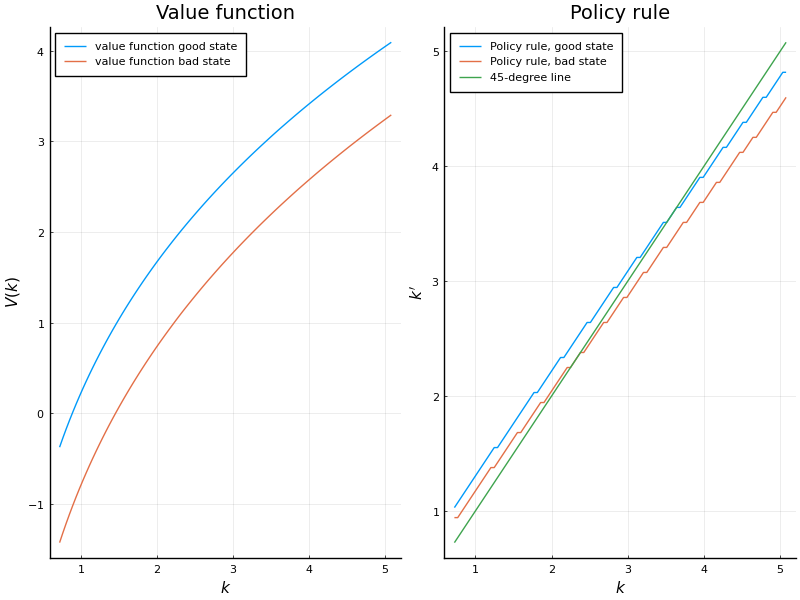
\includegraphics[width=0.8\linewidth]{plot_a.png}
		\end{center}
	\item Starting wlog at a good state ($z_g$).
		\begin{center}
			\textbf{b}\par\medskip
			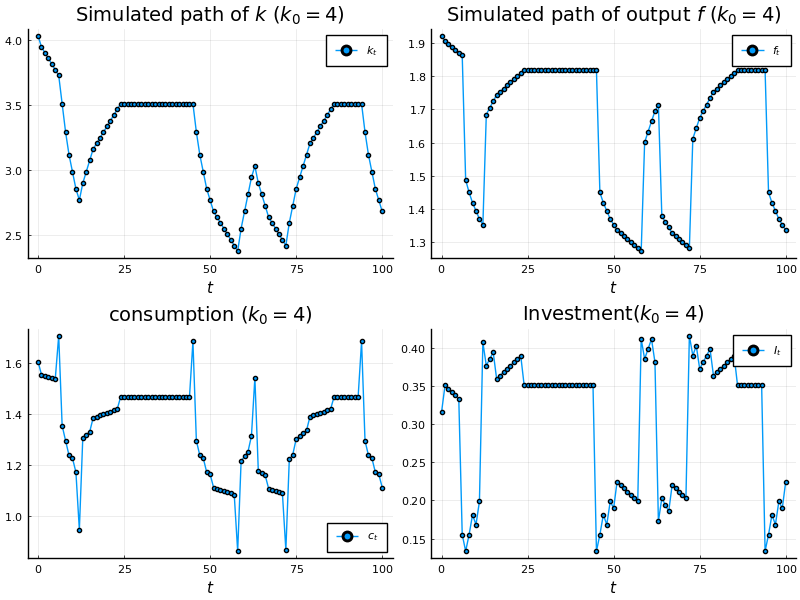
\includegraphics[width=0.8\linewidth]{plot_b.png}
		\end{center}



Value function iteration converged in 103 iterations (maxerr$=9.181072240238564e-7$)
\\\\
 $k_t:$ 
 \\mean = 2.992779237439736 
 \\std = 0.40788905355882615 
 \\std/mean 0.1362910596465402

 $f_t:$ 
\\ mean = 1.5697633490375587 
\\ std = 0.22300006991975804 
\\ std/mean 0.14205967419005047
\\
\\ $c_t:$ mean = 1.2713327347818022 
\\ std = 0.18204583542790553 
\\ std/mean 0.1431929112241021
\\
\\ $I_t:$ mean = 0.2984306142557566 
\\ std = 0.08861038959064496 
\\ std/mean 0.29692124520008323
\\\\
Thus we can see that investment has the greates volatility as measured by the coefficient of variation.
	\end{enumerate}
\end{enumerate} 

\end{document}


